
\subsection{Magnetars}

Magnetars are the neutron stars with unusually high magnetic fields. These have magnetic fields that are almost billion times more stronger than the typical neutron stars. The origin of this very high magnetic field is not full understood, but there have been theories like convective magnetohydrodynamic dynamo effect \citeauthorandyear{duncan_thompson}, or simply as a result of collapse of progenitors having very high magnetic fields. They have been a vast area of research mainly because of their strong magnetic fields of the order of \num{e15} G \citeauthorandyear{pulsar_strong_mag} , and also because they've been known for the cause of Gamma Ray Bursts (GRBs) and X-Ray Bursts (XRBs) and also Fast Radio Bursts (FRBs).\\

\begin{figure}
\centering
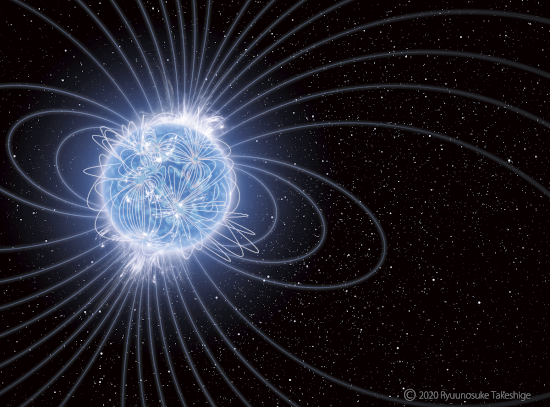
\includegraphics[height=0.5\textwidth, width=0.7\textwidth]{images/magnetar.png}
\caption{\small Artistics image of magnetic lines of a magnetar. Image by Ryuunosuke Takeshige}
\end{figure}

\subsubsection{Magnetars in Binary Systems}

It is still a mystery as to which stars get formed into Magnetars, and which process resulted in the extremely high magnetic field. In \citeauthorandyear{popov_binary_magnetar}, the author discusses the mechanism which might lead to the formation of such a binary system, and various other models that can be used to explain the existence of binary systems having magnetars. Following \citeauthorandyear{where_are_magnetar_binary_companion}, where they've conducted the experiment using photometry method of candidate magnetar counterparts to identify any bound companion stars among the Galactic population, they've estimated that 5 - 10 percent of the galactic population could plausibly have a bound magnetar companion. They've made the estimation assuming that the Magnetars are formed only through core collapse.

\begin{figure}[h]
\centering
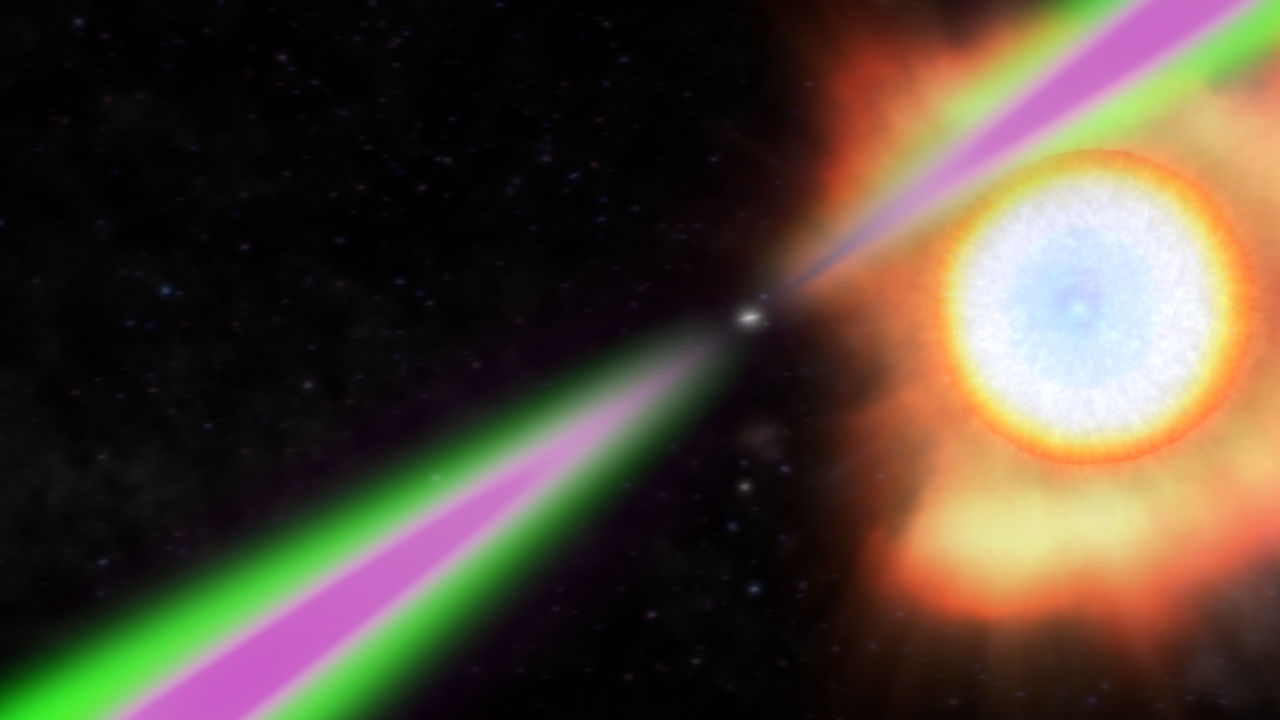
\includegraphics[height=0.4\textwidth, width=0.6\textwidth]{images/BWP.jpg}
\caption{\small Spinning 390 times a second, PSR J1311-3430 periodically swings its radio (green) and gamma-ray (magenta) beams past Earth in this artist's concept. The pulsar heats the facing side of its stellar partner to temperatures twice as hot as the sun's surface and slowly evaporates it. Credits NASA's Goddard Space Flight Center}
\end{figure}
